\section{Ejercicio 6}


\subsection{Desarrollo}
En este ejercicio se pide ejecutar el lote anterior con el scheduler FCFS
y compararlo con el ejercicio anterior con un solo procesador.


\subsection{Experimentación}
El gráfico de Gantt para el lote de tareas loteEj5.tsk se exhibe en la figura \ref{fig:ej6FCFS}. \par
\begin{figure}[H]
  \centering
    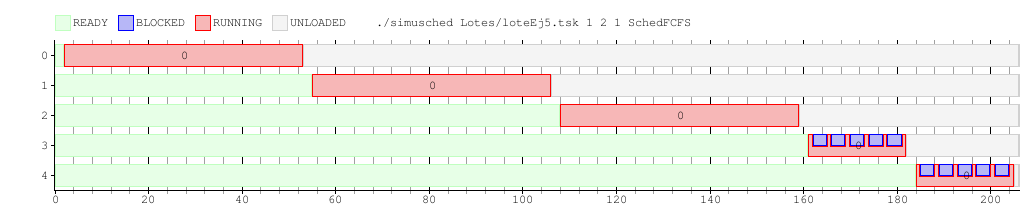
\includegraphics[width=1.1\textwidth]{imagenes/Ej6.png}
  \caption{loteEj5.tsk con FCFS}
  \label{fig:ej6FCFS}
\end{figure}
Podemos ver que el gráfico se asemeja mucho a la corrida del lote en \verb|SchedRR| con quantum 50. Volcamos los datos de tiempo en la tabla \ref{tab:ej6FCFS} de tiempos para cada tarea\par

\begin{table}
\centering
\begin{tabular}{ | c | c | c | c | c | c | c | }
  \hline			
  pid & ciclos & inicio & fin & latencia & waiting time & tiempo total  \\
  \hline
0 & 51 & 0 & 53 & 2 & 2 & 53\\
1 & 51 & 0 & 106 & 55 & 55 & 106\\
2 & 51 & 0 & 159 & 108 & 108 & 159\\
3 & 21 & 0 & 182 & 161 & 161 & 182\\
4 & 21 & 0 & 205 & 184 & 184 & 205\\
  \hline
promedio & - & - & - & 102 & CPU: 55  & CPU: 106 \\
                & &  &  &  & E/S: 172.5  & E/S: 193\\
\hline
\end{tabular}
\caption{Tiempos para loteEj5.tsk con FCFS}\label{tab:ej6FCFS}
\end{table}

FCFS y RR con quantum 50 tienen latencia promedio similares, y waiting times y tiempos totales similares también para los preceso de E/S, pues en ambos casos, corren últimos y luego de que hayan corrido los proceso más largo de CPU. En cambio para las tareas intensas de CPU, éstos dos últimos valores son mejores en FCFS, justamente porque éstos procesos corren primeros y completos antes de cambiar a las tareas de E/S.\par